%%%%%%%%%%%%%%%%%%%%%%%%%%%%%%%%%%%%%%%%%%%%%%%%%%%%%%%%%%%%%%%%%%%%%%%%%%%%%
%% Original default rstudio/pandoc latex file
%% upated by @jhollist 09/15/2014
%% inspired by @cboetting https://github.com/cboettig/template and
%% @rmflight blog posts:
%% http://rmflight.github.io/posts/2014/07/analyses_as_packages.html 
%% http://rmflight.github.io/posts/2014/07/vignetteAnalysis.html).  
%%%%%%%%%%%%%%%%%%%%%%%%%%%%%%%%%%%%%%%%%%%%%%%%%%%%%%%%%%%%%%%%%%%%%%%%%%%%%

\documentclass[11pt,]{article}
\usepackage[T1]{fontenc}
\usepackage{lmodern}
\usepackage{amssymb,amsmath}
\usepackage{ifxetex,ifluatex}
\usepackage{fixltx2e} % provides \textsubscript
% use upquote if available, for straight quotes in verbatim environments
\IfFileExists{upquote.sty}{\usepackage{upquote}}{}
\ifnum 0\ifxetex 1\fi\ifluatex 1\fi=0 % if pdftex
  \usepackage[utf8]{inputenc}
\else % if luatex or xelatex
  \ifxetex
    \usepackage{mathspec}
    \usepackage{xltxtra,xunicode}
  \else
    \usepackage{fontspec}
  \fi
  \defaultfontfeatures{Mapping=tex-text,Scale=MatchLowercase}
  \newcommand{\euro}{€}
\fi
% use microtype if available
\IfFileExists{microtype.sty}{\usepackage{microtype}}{}
\usepackage{longtable,booktabs}
\usepackage{graphicx}
% Redefine \includegraphics so that, unless explicit options are
% given, the image width will not exceed the width of the page.
% Images get their normal width if they fit onto the page, but
% are scaled down if they would overflow the margins.
\makeatletter
\def\ScaleIfNeeded{%
  \ifdim\Gin@nat@width>\linewidth
    \linewidth
  \else
    \Gin@nat@width
  \fi
}
\makeatother
\let\Oldincludegraphics\includegraphics
{%
 \catcode`\@=11\relax%
 \gdef\includegraphics{\@ifnextchar[{\Oldincludegraphics}{\Oldincludegraphics[width=\ScaleIfNeeded]}}%
}%
\ifxetex
  \usepackage[setpagesize=false, % page size defined by xetex
              unicode=false, % unicode breaks when used with xetex
              xetex]{hyperref}
\else
  \usepackage[unicode=true]{hyperref}
\fi
\hypersetup{breaklinks=true,
            bookmarks=true,
            pdfauthor={},
            pdftitle={Associations between Chlorophyll a and various Microcystin-LR Health Advisory Concentrations},
            colorlinks=true,
            citecolor=blue,
            urlcolor=blue,
            linkcolor=magenta,
            pdfborder={0 0 0}}
\urlstyle{same}  % don't use monospace font for urls
\setlength{\parindent}{0pt}
\setlength{\parskip}{6pt plus 2pt minus 1pt}
\setlength{\emergencystretch}{3em}  % prevent overfull lines
\setcounter{secnumdepth}{5}

%%%%%%%%%%%%%%%%%%%%%%%%%%%%%%%%%%%%%%%%%%%%%%%%%%%%%%%%
%Changes borrowed from @cboettig, added by @jhollist 
% A modified page layout 
\textwidth 6.75in
\oddsidemargin -0.15in
\evensidemargin -0.15in
\textheight 9in
\topmargin -0.5in
\usepackage{lineno} % add 
%%%%%%%%%%%%%%%%%%%%%%%%%%%%%%%%%%%%%%%%%%%%%%%%%%%%%%%%

%%%%%%%%%%%%%%%%%%%%%%%%%%%%%%%%%%%%%%%%%%%%%%%%%%%%%%%%
%%Packages and layout changes by @jhollist 09/15/2014
\usepackage{ragged2e}
\usepackage[font=normalsize]{caption}
  \usepackage[doublespacing]{setspace}
\usepackage{parskip}
\usepackage{fancyhdr}
\pagestyle{fancy}
\fancyhf{}
\renewcommand{\headrulewidth}{0pt}
\rfoot{\today}
\lfoot{\thepage}
%%Changed default abstract width and added lines
\renewenvironment{abstract}{
  \hfill\begin{minipage}{1\textwidth}
  \rule{\textwidth}{1pt}\vspace{5pt}
  \normalsize
  \begin{justify}
  \bfseries\abstractname\vspace{5pt}
  \end{justify}}
  {\par\noindent\rule{\textwidth}{1pt}\end{minipage}
}
%%%%%%%%%%%%%%%%%%%%%%%%%%%%%%%%%%%%%%%%%%%%%%%%%%%%%%%%

\title{Associations between Chlorophyll \emph{a} and various Microcystin-LR
Health Advisory Concentrations}
\author{
Jeffrey W. Hollister
Betty J. Kreakie
Dorothy Q. Kellog
}
\date{}

\begin{document}
%%Edited by @jhollist 09/15/2014
%%Adds title from YAML
\begin{singlespace}
\begin{center}
\huge Associations between Chlorophyll \emph{a} and various Microcystin-LR
Health Advisory Concentrations
\end{center}
%%Adds Author, correspond email asterisk, and affilnum from YAML
\begin{center}
\large
Jeffrey W. Hollister \textsuperscript{*} \textsuperscript{1} 
Betty J. Kreakie \textsuperscript{1} 
Dorothy Q. Kellog \textsuperscript{2} 
\end{center}
%%Adds affiliations from YAML
\begin{justify}
\footnotesize \emph{ 
\\*
\textsuperscript{1}US Environmental Protection Agency, Office of Research and Development,
National Health and Environmental Effects Research Laboratory, Atlantic
Ecology Division, 27 Tarzwell Drive Narragansett, RI, 02882, USA\\*
\\*
\textsuperscript{2}University of Rhode Island, Department of Natural Resources Science,
Kingston, RI, 02882, USA\\*
}
%%Adds corresponding author email(s) from YAML
\newcounter{num}
\setcounter{num}{1}
\\[0.1cm]
\footnotesize \emph{ 
\ifnum\value{num}=1%
\textsuperscript{*} corresponding author:
\fi
\href{mailto:hollister.jeff@epa.gov}{\nolinkurl{hollister.jeff@epa.gov}}
\stepcounter{num}
}
\end{justify}
%%Adds date from YAML
\normalsize

\end{singlespace}


\singlespace

\vspace{2mm}

\hrule

Cyanobacteria harmful algal blooms (cHABs) are associated with a wide
range of adverse health effects that stem mostly from the presence of
cyanotoxins. To help protect against these impacts, several health
advisory levels have been set for some toxins. In particular, one of the
more common toxins, microcystin, has several advisory levels set for
drinking water and recreational use and managing water bodies to meet
those levels could have far reaching benefits. However, compared to
other water quality measures, measurements of microcystin are not common
and current field measurement techniques have limited precision and
accuracy. Addressing these issues will take time and resourced. Thus,
there is utility in finding indicators of microcystin that are already
widely available, can be estimated quickly and \emph{in situ}, and used
as a first defense against high levels of microcystin. In particular,
chlorophyll \emph{a} is very commonly measured, can be estimated
\emph{in situ}, and has been shown to be positively associated with
microcystin. In this paper we use this association to provide estimates
of chlorophyll \emph{a} that if exceeded would be indicative of a higher
probability of exceeding select health advisory concentrations for
microcystin-LR. Using the 2007 National Lakes Assessment and a
conditional probability approach that has been used in other water
quality settings, we identify chlorophyll \emph{a} concentrations that
are more likely than not to be associated with an exceedance of a
microcystin health advisory level. We look at the recent US EPA
standards for drinking water as well as the World Health Organization
levels for drinking water and recreational use. For microcystin
concentrations of 0.3, 1, 1.6, and 2 we find chlorophyll \emph{a}
concentrations of 25.1, 69.6, 84.96, and 113.14, respectively. When
managing for these various microcystin levels exceeding these reported
chlorophyll \emph{a} concentrations should be a trigger for further
testing and possible management action.

\vspace{3mm}

\hrule

\doublespace

\section{Introduction}\label{introduction}

In the summer of 2014, the city of Toledo, OH was forced to shut down
their municipal water supply due in part to an excess of Microcystin-LR
that resulted from a ongoing cyanobacteria harmful algal bloom (cHAB) in
Lake Erie. Since this event, significant legislation has been passed in
the United States and the US Environmental Protection Agency (USEPA) has
released suggested microcystin-LR concentrations that would trigger
health advisories. While these levels and associated advisories are
likely to help mitigate the impacts from harmful algal blooms, they are
not without complications.

One of these complications is that they rely on available measurements
of microcystin-LR. This toxin can be measured in the field using test
strips but these are a coarse measure at best and currently available
test strips focus on 1 and 10 \(\mu\)g/L {[}REFS{]}. Measurements with
greater accuracy and precision requires taking regular water samples and
having those samples process in a lab to determine the toxin
concentration {[}REFS{]}. This has the potentially to be costly and time
consuming both factors which could limit monitoring efforts.
Fortunately, microcystin-LR has been shown to be associated with several
other, more easily measured components of water quality.

Chlorophyll \emph{a} is a very commonly measured components of water
quality that is also known to be associated with Microsystin-LR
concentrations {[}REFS{]}. Additionally there are many rapid
measurements for assessing chlorophyll \emph{a} levels \emph{in situ}.
For instance, there are small or hand held flourometers that provide
reliable measurements {[}REFS{]}. Given these facts, it might be
possible to identify chlorophyll \emph{a} concentrations that would be
associated with the various Microcystin-LR health advisory levels.
Identifying these associations would provide another reliable tool for
water resource managers to use to help manage the threat to public
health posed by cHABs.

Use association and cpa to id chl a concentration that indicative of
exceeding HA

\section{Methods}\label{methods}

\begin{longtable}[c]{@{}lll@{}}
\toprule
\begin{minipage}[b]{0.11\columnwidth}\raggedright\strut
Source
\strut\end{minipage} &
\begin{minipage}[b]{0.16\columnwidth}\raggedright\strut
Type
\strut\end{minipage} &
\begin{minipage}[b]{0.19\columnwidth}\raggedright\strut
Concentration
\strut\end{minipage}\tabularnewline
\midrule
\endhead
\begin{minipage}[t]{0.11\columnwidth}\raggedright\strut
WHO
\strut\end{minipage} &
\begin{minipage}[t]{0.16\columnwidth}\raggedright\strut
Drinking
\strut\end{minipage} &
\begin{minipage}[t]{0.19\columnwidth}\raggedright\strut
1 ug/l
\strut\end{minipage}\tabularnewline
\begin{minipage}[t]{0.11\columnwidth}\raggedright\strut
U.S. EPA
\strut\end{minipage} &
\begin{minipage}[t]{0.16\columnwidth}\raggedright\strut
Drinking
\strut\end{minipage} &
\begin{minipage}[t]{0.19\columnwidth}\raggedright\strut
0.3 ug/l
\strut\end{minipage}\tabularnewline
\begin{minipage}[t]{0.11\columnwidth}\raggedright\strut
U.S. EPA
\strut\end{minipage} &
\begin{minipage}[t]{0.16\columnwidth}\raggedright\strut
Drinking
\strut\end{minipage} &
\begin{minipage}[t]{0.19\columnwidth}\raggedright\strut
1.6 ug/l
\strut\end{minipage}\tabularnewline
\begin{minipage}[t]{0.11\columnwidth}\raggedright\strut
WHO
\strut\end{minipage} &
\begin{minipage}[t]{0.16\columnwidth}\raggedright\strut
Recreational
\strut\end{minipage} &
\begin{minipage}[t]{0.19\columnwidth}\raggedright\strut
2-4 ug/l
\strut\end{minipage}\tabularnewline
\begin{minipage}[t]{0.11\columnwidth}\raggedright\strut
WHO
\strut\end{minipage} &
\begin{minipage}[t]{0.16\columnwidth}\raggedright\strut
Recreational
\strut\end{minipage} &
\begin{minipage}[t]{0.19\columnwidth}\raggedright\strut
10-20 ug/l
\strut\end{minipage}\tabularnewline
\begin{minipage}[t]{0.11\columnwidth}\raggedright\strut
WHO
\strut\end{minipage} &
\begin{minipage}[t]{0.16\columnwidth}\raggedright\strut
Recreational
\strut\end{minipage} &
\begin{minipage}[t]{0.19\columnwidth}\raggedright\strut
20-2000 ug/l
\strut\end{minipage}\tabularnewline
\begin{minipage}[t]{0.11\columnwidth}\raggedright\strut
WHO
\strut\end{minipage} &
\begin{minipage}[t]{0.16\columnwidth}\raggedright\strut
Recreational
\strut\end{minipage} &
\begin{minipage}[t]{0.19\columnwidth}\raggedright\strut
\textgreater{}2000 ug/l
\strut\end{minipage}\tabularnewline
\bottomrule
\end{longtable}

We evaluated associated chlorophyll \emph{a} concentrations for an
effect for each of the WHO and EPA levels. Lakes with higher
microcystin-LR concentrations were rare. Only 1.1616651 \% of lakes
sampled had a concentration greater than 10. For this analysis we focus
on the microcystin concentrations that are better represented in the NLA
data. These were 0.3, 1, 1.6, and 2 \(\mu\)g/L.

\section{Results}\label{results}

\begin{longtable}[c]{@{}lll@{}}
\toprule
\begin{minipage}[b]{0.13\columnwidth}\raggedright\strut
Source
\strut\end{minipage} &
\begin{minipage}[b]{0.18\columnwidth}\raggedright\strut
Microcystin
\strut\end{minipage} &
\begin{minipage}[b]{0.18\columnwidth}\raggedright\strut
Chlorophyll
\strut\end{minipage}\tabularnewline
\midrule
\endhead
\begin{minipage}[t]{0.13\columnwidth}\raggedright\strut
EPA\_Child
\strut\end{minipage} &
\begin{minipage}[t]{0.18\columnwidth}\raggedright\strut
0.3
\strut\end{minipage} &
\begin{minipage}[t]{0.18\columnwidth}\raggedright\strut
25.1
\strut\end{minipage}\tabularnewline
\begin{minipage}[t]{0.13\columnwidth}\raggedright\strut
WHO
\strut\end{minipage} &
\begin{minipage}[t]{0.18\columnwidth}\raggedright\strut
1
\strut\end{minipage} &
\begin{minipage}[t]{0.18\columnwidth}\raggedright\strut
69.6
\strut\end{minipage}\tabularnewline
\begin{minipage}[t]{0.13\columnwidth}\raggedright\strut
EPA\_Adult
\strut\end{minipage} &
\begin{minipage}[t]{0.18\columnwidth}\raggedright\strut
1.6
\strut\end{minipage} &
\begin{minipage}[t]{0.18\columnwidth}\raggedright\strut
84.96
\strut\end{minipage}\tabularnewline
\begin{minipage}[t]{0.13\columnwidth}\raggedright\strut
WHO
\strut\end{minipage} &
\begin{minipage}[t]{0.18\columnwidth}\raggedright\strut
2
\strut\end{minipage} &
\begin{minipage}[t]{0.18\columnwidth}\raggedright\strut
113.1
\strut\end{minipage}\tabularnewline
\bottomrule
\end{longtable}

\section{Discussion}\label{discussion}

\section{Figures}\label{figures}

\begin{figure}[htbp]
\centering
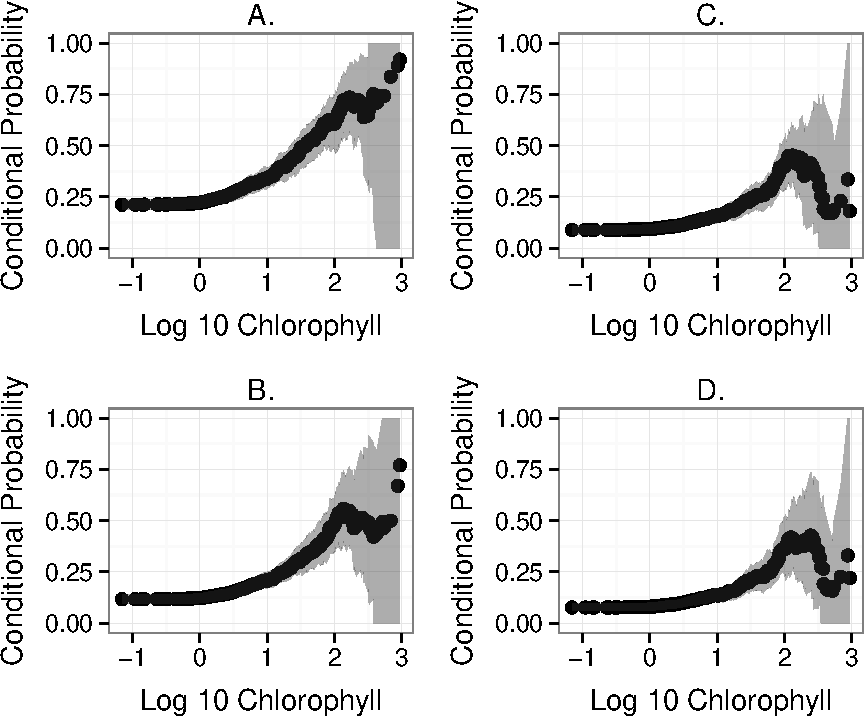
\includegraphics{manuscript_files/figure-latex/epa_child_cp_plot-1.pdf}
\caption{}
\end{figure}

\newpage

\begin{figure}[htbp]
\centering
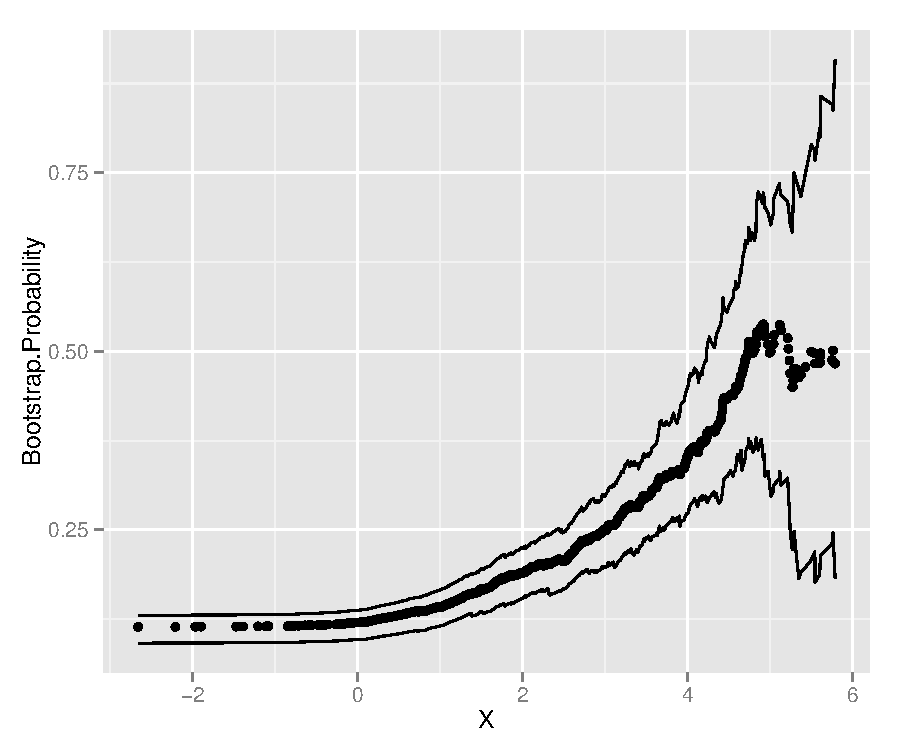
\includegraphics{manuscript_files/figure-latex/who_drink_cp_plot-1.pdf}
\caption{}
\end{figure}

\newpage

\begin{figure}[htbp]
\centering
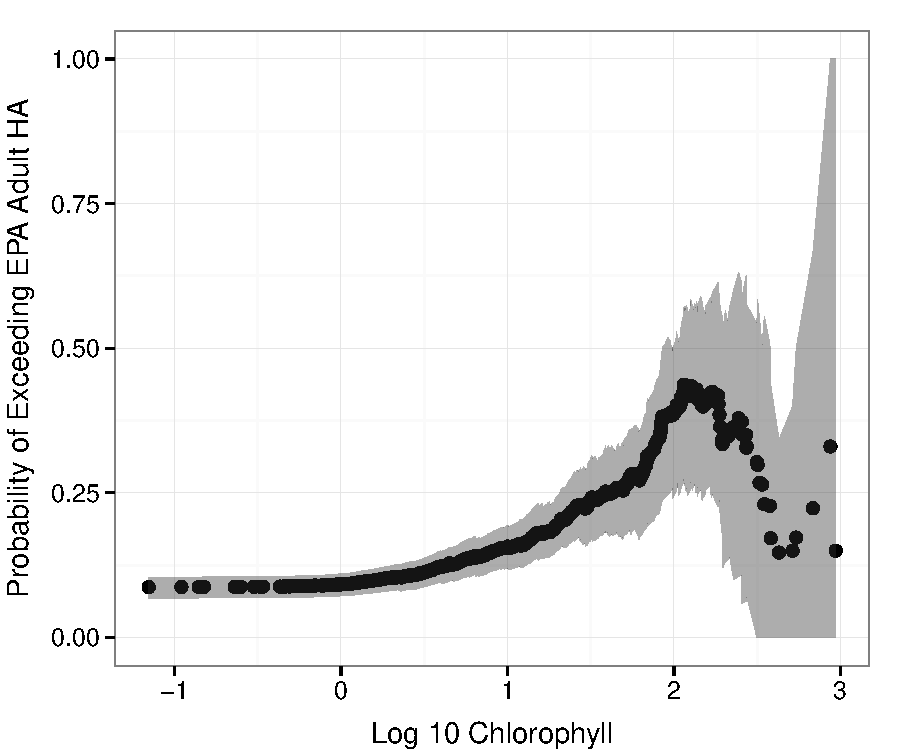
\includegraphics{manuscript_files/figure-latex/epa_adult_cp -1.pdf}
\caption{}
\end{figure}

\newpage

\begin{figure}[htbp]
\centering
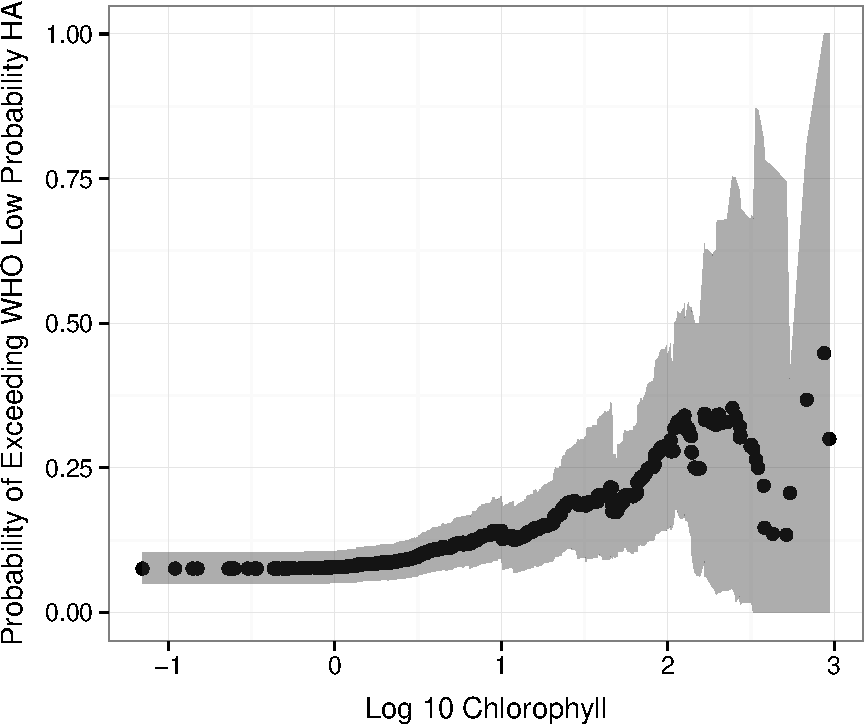
\includegraphics{manuscript_files/figure-latex/who_rec_low1_cp-1.pdf}
\caption{}
\end{figure}

\newpage

\section*{References}\label{references}
\addcontentsline{toc}{section}{References}

\end{document}